    The topic of artificial intelligence is known as a fast-developing field, which can be assessed through the growth of the number of AI journal publications. For example, from $2019$ to $2020$ the number of AI journal publications has grown by a factor of $1.345$; in comparison to the growth rate of $1.196$ from $2018$ to $2019$ \cite{zhang2021ai}. Still, the most commonly used algorithms are linear and logistic regression directly followed by decision trees or random forests \cite{state_of_data_science_2021}. While the first kind of model fails when features are correlated in a non-linear way, decision trees have the expressive power to solve such types of problems \cite{molnar2020interpretable}. 
    
    This basic type of algorithm remains popular, as they can produce models with a high bias, and this is also a property that makes them model-inherent interpretable. Furthermore, they are the basic building blocks for more complex models created through bagging or boosting. Two good examples for boosting are AdaBoost (i.e., with decision trees as estimators) and Gradient Boosting. Among other models, random forests are a well-known bagging model. All these learning methods make use of tree-based models and are supervised algorithms. Therefore, this section introduces tree-based models but uses a visual approach (like in \cite{dtreeviz}) referred to later in this thesis. 
    
    \paragraph{General Concept} Regardless of what kind of tree-based model is used, the input space $\mathbb{I}$ is partitioned into distinct cuboids $R_1,...,R_T \subset \mathbb{I}$ ($T \in \mathbb{N}$ the number of cuboids). Each of these cuboids $R_t$ are assigned a model ($t \in [1,...,T]$) \cite{bishop2006pattern}. For example, when using standard decision trees, constant models $M_{c_t}: R_t \to \mathbb{T}$ with $r \mapsto c_t$ are used, such that all inputs $r \in R_t$ are assigned the constant $c_t \in \mathbb{T}$. This kind of partitioning in combination with the assigned predictions $c_t$ is visualized in Figure \ref{fig:sigmoid_partitioning_decision_tree} using the model from the example \ref{Bsp:sigmoid_estimation_example}.
    
    \begin{figure}[H]
        \centering
        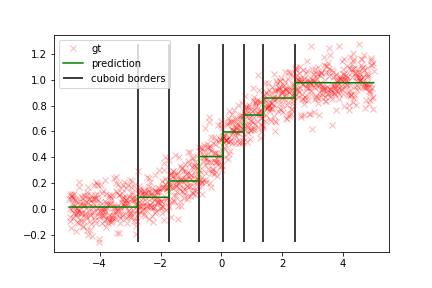
\includegraphics[width=9cm]{images/ml_basics/sigmoid_depth3.png}\caption{Partitioning of the one-dimensional input space given a decision tree trained to approximate the sigmoid function}
        \label{fig:sigmoid_partitioning_decision_tree}
    \end{figure}
    
    Training a tree-based model is, therefore ,twofold: (i) Partitioning the input space, and (ii) assigning each cuboid a model. The input space is partitioned by learning a function $\mathcal{T}: \mathbb{I} \to [1,...,T]$, which assigns each $x \in \mathbb{I}$ a cuboid $R_t$. 

    $\mathcal{T}$ is represented as a binary tree. Each leaf of the tree refers to a cuboid, $R_t$ and all the other nodes are split nodes. A split node $n_{d,u}$ has two child nodes $n_{(d+1),l}$, $n_{(d+1),r}$ and is coupled with a split criterion $f_k~\leq~ \theta_{d,u}$ ($k \in [1,...,K]$, $K$ is the number of available features, $n_{d,u}$ refers to the $u$'th node on the depth $d$ and $\theta_{d,u}$ is a parameter comparable with $f_k$). 
    Given a sample $(\mathbf{x}_i, t_i)$,  the split criterion is evaluated via 
    \begin{gather}
        (\mathbf{x}_i \models f_k~\leq~\theta_{i,u}) \Longleftrightarrow (x_{i,k} ~\leq~\theta_u) \label{formular_split_criterion}
    \end{gather}
    If $\mathbf{x}_i$ is a model for the split criterion, then the procedure continues with $n_{(d+1),r}$ otherwise with $n_{(d+1),l}$. When a leaf referring to a cuboid $R_t$ is reached by following this procedure from the root node $n_{1,1}$, the output of $\mathcal{T}(\mathbf{x}_i)$ is known to be $t$. Depending on the implementation, operators other than $\leq$ may be allowed.

    In general, finding the optimal $\mathcal{T}$ is infeasible as the structure of the tree and the parameters of each node need to be found, which spans a solution space that grows exponentially with the number of nodes available for $\mathcal{T}$.
    
    In the case of decision trees, a greedy approach is used to learn $\mathcal{T}$ and, therefore, the solution might not be optimal. This work is centered around explaining and interpreting models with respect to semantic constraint validation. Consequently, it is unavoidable to understand the basic approach used to train a decision tree.

    \paragraph{Greedy Inducer} Here, a decision tree used for regression with cuboid borders, as visualized in Figure \ref{fig:sigmoid_partitioning_decision_tree}, should be learned. The process is a recursive one, and in each step, there is a set of samples $R_{d,u} \subset D$ and one needs to decide whether the node $n_{d,u}$ corresponding to the step will be a leaf node or a split node. This criterion needs to be chosen wisely, as shown in example \ref{Bsp:sigmoid_estimation_example}. In the case of a regression task, one might stop if all the samples $(\mathbf{x}_i,t_i) \in R_{d,u}$ have the same target value $t_i$ or the target values have a limited standard deviation. The first criterion will lead to decision trees with high variance because the decision trees will be specialized to the dataset used for training. The second criterion requires further knowledge about the dataset, and the standard deviation might be different in various spaces of the dataset. In this example, the inducer decides that the node will be a leaf node if, $d = 4$ as example \ref{Bsp:sigmoid_estimation_example} has shown that a maximal depth of $4$ is reasonable for the given task. 
    
    If $n_{d,u}$ will be a leaf node, a constant model $M_{c_{d,u}}$ has to be selected such that the performance of the model is as good as possible, given the available data $R_{d,u}$. As typical for regression tasks, the performance is measured by the mean squared error:
    \begin{gather}
        P(M_{c_{d,u}}, R_{d,u}) = \frac{1}{|R_{d,u}|} \sum_{(\mathbf{x}_i,t_i) \in R_{d,u}} (t_i - c_{d,u})^2 \label{mean_squared_error}
    \end{gather}
    minimizing the term with respect to $c_{d,u}$ leads to the optimal solution, which is the average:
    \begin{gather}
        c_{d,u} = \frac{1}{|R_{d,u}|} \sum_{(\mathbf{x}_i,t_i) \in R_{d,u}} t_i \label{optimal_predication_maximum_likelihood}
    \end{gather}
    As a leaf is reached, $R_{d,u}$ corresponds to a cuboid $R_t$, which is referred to by $\mathcal{T}$. The feature vectors corresponding to the samples in $R_{d,u}$ form a subset of $R_t$, which will be real in most cases. That is because $R_t$ represents the cuboid of all possible feature vectors $x_i$ that get the prediction $c_t$ assigned due to $\mathcal{T}(\mathbf{x}_i) = t$ and $R_{d,u}$ is just the subset of the samples of $D$ used to infer the leaf and $c_t$ during training.

    If $n_{d,u}$ will be a split node, the data $R_{d,u}$ has to be split into disjoint sets $R_{(d+1),l}$ and $R_{(d+1),r}$ given a criterion $f_k \leq \theta_{d,u}$ as described above. $f_k$ and $\theta_{d,u}$ are chosen by trying all features for all possible splitting values and choosing the one maximizing the performance of the sum of the child nodes, measured by formula \ref{mean_squared_error}. The calculation is performed with the optimal prediction $c_{(d+1),l}$ and $c_{(d+1),r}$ calculated with (\ref{optimal_predication_maximum_likelihood}). Then the procedure is recursively called for $n_{(d+1),l}$ and $n_{(d+1),r}$.
    
    Finally, the training of a decision tree is just a matter of starting the recursive procedure for the root node $n_{1,1}$ with the data $R_{1,1} := D$.
    
    \begin{Bsp}{Estimating the $R_{d,u}$ of the motivating example decision tree}{motivating_example_rdu_estimation}
    Here, the recursive procedure described is applied to discover the sets $R_{d,u}$ given the dataset $D$ shown in example \ref{Bsp:sample-to-node_mapping_motivating_example} and the decision tree in Figure \ref{motivating_example_decision_tree}. Starting with the root node $n_{1,1}$ (Node 0 in Figure \ref{motivating_example_decision_tree}), for which $R_{1,1} = D$ is given, the examples are split according to the criterion: $\text{allergic\_to} \leq 0$ (using formula \ref{formular_split_criterion}). To give $R_{2,1}$ and $R_{2,2}$. Next, the procedure would be called for $n_{2,1}$. Executing the procedure until the end, gives for each node $n_{d,u}$ the indices of $D$ occurring in $R_{d,u}$. The result is shown in Figure \ref{fig:example_instance_to_node_assignment_table}; additionally referring to the persons and the enumeration of the nodes in Figure \ref{motivating_example_decision_tree}.
    
    \captionsetup{type=htypei}
    \begin{minipage}[t]{\linewidth}
        \vspace{1ex}
        \centering
        \begin{tabular}{ll|lll}
            \toprule
             Node & $n_{d,u}$ & Persons & $\{i \mid (x_i,t_i) \in R_{d,u}\}$ \\
             \midrule
             $0$ & $n_{1,1}$ & \uri{:Max}, \uri{:Maria}, \uri{:Eva}, \uri{:Laura}& $[1,...,9999]$ \\
             $1$ & $n_{2,1}$ & \uri{:Maria}, \uri{:Eva}& $[3334,...,9166]$ \\
             $4$ & $n_{2,2}$ & \uri{:Max}, \uri{:Laura}& $[1,...,3334] \cup [9167,...,9999]$ \\
             $2$ & $n_{3,1}$ & \uri{:Eva} & $[4167,...,9166]$ \\
             $3$ & $n_{3,2}$ & \uri{:Maria} & $[3334,...,4166]$ \\
             \bottomrule
        \end{tabular}
        \captionof{table}{For each node $n_{d,u}$ in Figure \ref{motivating_example_decision_tree}, the indices of the dataset $D$ included in $R_{d,u}$ are shown}
        \label{fig:example_instance_to_node_assignment_table}
        \vspace{1ex}
    \end{minipage}
\end{Bsp}
    
    The model's training procedure stays the same when a decision tree for classification is trained. Besides that, the performance measure changes from the mean squared error to the \emph{negative cross-entropy} or the \emph{Gini index} and, therefore, the optimal prediction changes to be the target class referred to by the most examples in the node.
    
    \paragraph{Visually interpreting the Decision Tree} This work builds on the kind of visualizations shown in Figure \ref{motivating_example_decision_tree} and \ref{fig:sigmoid_dtree} proposed by the \texttt{dtreeviz} library \cite{dtreeviz}. The visualizations are built to explain what has been learned by the decision tree and why the decision tree makes a certain decision given a problem instance. This is done with respect to a specific dataset $D$.
    
    For each node $n_{d,u}$\footnote{The indexing is demonstrated for some nodes in the Figure \ref{fig:sigmoid_dtree}}, the distribution of the ground truth values of the set of samples $R_{d,u}$ is visualized. As described above, $R_{d,u}$ refers to the samples used to decide whether the node $n_{d,u}$ will be a split or a leaf node given the dataset $D$. In the case that $n_{d,u}$ is a split node, the distribution of the ground truth is shown with respect to the split feature $f_k$. As the values of the other features are ignored, the distribution shows the marginal effect the feature has on the ground truth. Further, the size of distributions is scaled with the number of samples included in $R_{d,u}$. 
    
    Next, to explain why the decisions are made by the decision tree induced by the learning algorithm during training, Figure \ref{fig:sigmoid_dtree} is investigated further.
    
    Figure \ref{fig:sigmoid_dtree} shows the decision tree trained to approximate the sigmoid function from example \ref{Bsp:sigmoid_estimation_example}, the explanation will be about the regression task but can be transferred analog to the classification task.
    In the case of regression, scatter plots are used to show the distribution of the points $\{(\mathbf{x}_{i,k},t_i) \mid (\mathbf{x}_i,t_i) \in R_{d,u})\}$ per split node.
    Starting at the root node $n_{1,1}$ with $R_{1,1} = D$, the learning algorithm had to choose the split feature and the decision boundary for each split node. In example \ref{Bsp:sigmoid_estimation_example} only one feature $x$ is used. $x$ is the input to the sigmoid function, and will be the split feature for each split node. Hence, the split criterion for all nodes is $x \leq \theta_{d,u}$ and $\theta_{d,u}$ has the value shown right under the marker at the x-axis.
    Now it is visually verifiable that $\theta_{d,u}$ is chosen correctly and, thus, the performance
    \[- (P(M_{c_l}, R_{d,l}) + P(M_{c_r}, R_{d,r}))\] is maximized. Therefore, explaining the decision made at each split node is a matter of visually verifying that the new cuboid border shown by the vertical dotted line is chosen optimally. The horizontal dotted line corresponds to the optimal predictions, which would be given if the child nodes were leaves.
    
    In the case of regression, the optimal predictions of the learning algorithm estimated for each node can be verified as the horizontal dotted lines visualize them. In the leaves, the horizontal dotted line directly corresponds to the predictions made. 
    
    As a final note: For these visualizations to work and explain why specific cuboid borders are chosen, and the decision tree makes particular predictions, the dataset used for visualization should be the one initially used to train the decision tree. If a different dataset is used, the visualization will show how the decision tree behaves with respect to the new data, but will not show how the cuboid boundaries are chosen during the training process.
    
    \begin{figure}
        \centering
        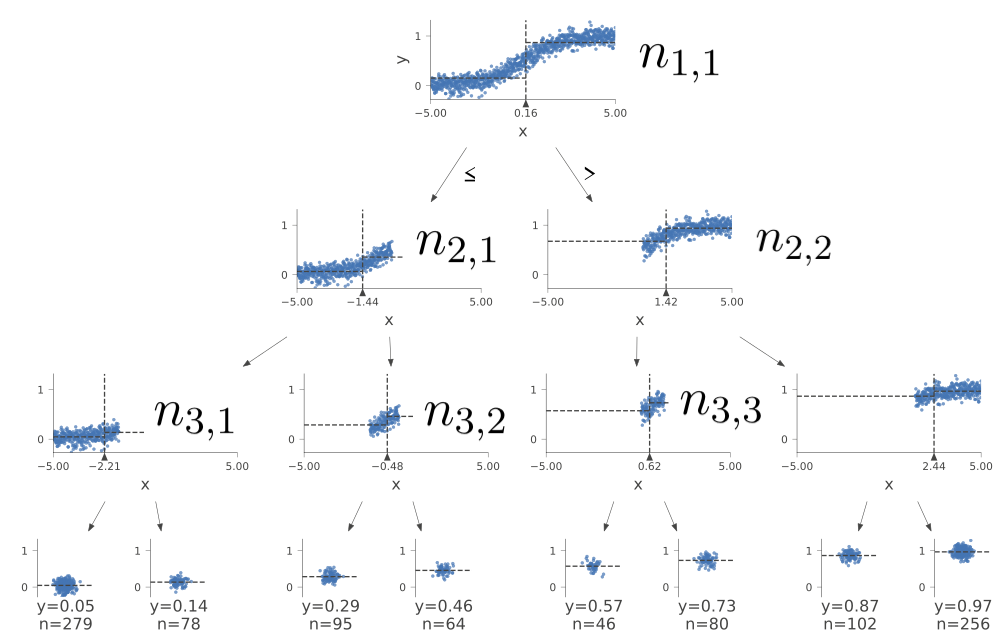
\includegraphics[width=12cm]{images/ml_basics/sigmoid_dtree.png}
        \caption{Visualization of a decision tree trained to approximate the sigmoid function with a maximal depth of four}
        \label{fig:sigmoid_dtree}
    \end{figure}